% ****** Start of file apssamp.tex ******
%
%   This file is part of the APS files in the REVTeX 4.1 distribution.
%   Version 4.1r of REVTeX, August 2010
%
%   Copyright (c) 2009, 2010 The American Physical Society.
%
%   See the REVTeX 4 README file for restrictions and more information.
%
% TeX'ing this file requires that you have AMS-LaTeX 2.0 installed
% as well as the rest of the prerequisites for REVTeX 4.1
%
% See the REVTeX 4 README file
% It also requires running BibTeX. The commands are as follows:
%
%  1)  latex apssamp.tex
%  2)  bibtex apssamp
%  3)  latex apssamp.tex
%  4)  latex apssamp.tex
%
\documentclass[%
 reprint,
%superscriptaddress,
%groupedaddress,
%unsortedaddress,
%runinaddress,
%frontmatterverbose, 
%preprint,
%showpacs,preprintnumbers,
%nofootinbib,
%nobibnotes,
%bibnotes,
 amsmath,amssymb,
 aps,
%pra,
%prb,
%rmp,
%prstab,
%prstper,
%floatfix,
10.5pt,
]{revtex4-1}

\usepackage{graphicx}% Include figure files
\usepackage{subfigure}
\usepackage{multirow}
\usepackage{array}
\usepackage{dcolumn}% Align table columns on decimal point
\usepackage{bm}% bold math
%\usepackage{hyperref}% add hypertext capabilities
%\usepackage[mathlines]{lineno}% Enable numbering of text and display math
%\linenumbers\relax % Commence numbering lines

%\usepackage[showframe,%Uncomment any one of the following lines to test 
%%scale=0.7, marginratio={1:1, 2:3}, ignoreall,% default settings
%%text={7in,10in},centering,
%%margin=1.5in,
%%total={6.5in,8.75in}, top=1.2in, left=0.9in, includefoot,
%%height=10in,a5paper,hmargin={3cm,0.8in},
%]{geometry}

\usepackage{xeCJK}
%\setCJKmainfont[ItalicFont={KaiTi}, BoldFont={KaiTi}]{KaiTi}
\usepackage{textcomp}
\usepackage{chemfig}
\usepackage[version=4]{mhchem}
\usepackage{fontspec}
\usepackage{listings}
\usepackage{amsmath}
\usepackage{xcolor} % 定制颜色
\definecolor{mygreen}{rgb}{0,0.6,0}
\definecolor{mygray}{rgb}{0.5,0.5,0.5}
\definecolor{mymauve}{rgb}{0.58,0,0.82}
\lstset{
backgroundcolor=\color{white},      % choose the background color
basicstyle=\footnotesize\ttfamily,  % size of fonts used for the code
columns=fullflexible,
tabsize=4,
breaklines=true,               % automatic line breaking only at whitespace
captionpos=b,                  % sets the caption-position to bottom
commentstyle=\color{mygreen},  % comment style
escapeinside={\%*}{*)},        % if you want to add LaTeX within your code
keywordstyle=\color{blue},     % keyword style
stringstyle=\color{mymauve}\ttfamily,  % string literal style
frame=single,
rulesepcolor=\color{red!20!green!20!blue!20},
% identifierstyle=\color{red},
language=Mathematica,
}

\usepackage[normalem]{ulem}

\newcommand{\chuhao}{\fontsize{42pt}{44.9pt}\selectfont}    % 初号, 1.5倍行距
\newcommand{\xiaochu}{\fontsize{30pt}{40pt}\selectfont}    % 小初, 1.5倍行距
\newcommand{\yihao}{\fontsize{26pt}{36pt}\selectfont}    % 一号, 1.4倍行距
\newcommand{\erhao}{\fontsize{22pt}{28pt}\selectfont}    % 二号, 1.25倍行距
\newcommand{\xiaoer}{\fontsize{18pt}{18pt}\selectfont}    % 小二, 单倍行距
\newcommand{\sanhao}{\fontsize{16pt}{24pt}\selectfont}    % 三号, 1.5倍行距
\newcommand{\xiaosan}{\fontsize{15pt}{22pt}\selectfont}    % 小三, 1.5倍行距
\newcommand{\sihao}{\fontsize{14pt}{21pt}\selectfont}    % 四号, 1.5倍行距
\newcommand{\sihaox}{\fontsize{14pt}{28pt}\selectfont}    % 四号, 1.5倍行距
\newcommand{\banxiaosi}{\fontsize{13pt}{19.5pt}\selectfont}    % 半小四, 1.5倍行距
\newcommand{\xiaosix}{\fontsize{12pt}{24pt}\selectfont} 	% 小四, 1.5倍行距
\newcommand{\xiaosi}{\fontsize{12pt}{18pt}\selectfont}     
\newcommand{\dawuhao}{\fontsize{11pt}{11pt}\selectfont}    % 大五号, 单倍行距
\newcommand{\wuhao}{\fontsize{10.5pt}{10.5pt}\selectfont}    % 五号, 单倍行距
\newcommand{\xiaowu}{\fontsize{9pt}{9pt}\selectfont}    % 五号, 单倍行距

%\usepackage[fntef]{ctexcap}
%\CTEXsetup[number={\chinese{section}、},format={\Large\bfseries}]{section}
%\setCJKfamilyfont{fangsong}{FangSong}                      %仿宋2312 fs  
%\newcommand{\fangsong}{\CJKfamily{fangsong}}  

\usepackage{wrapfig}
\usepackage{fancyhdr}
\usepackage{fancybox}   


\usepackage{tikz}
\usepackage{circuitikz}



\newcommand{\bra}[1]{\langle #1 |}
\newcommand{\ket}[1]{| #1 \rangle}
\newcommand{\bracket}[2]{\langle #1 | #2 \rangle}
\newcommand{\bracketl}[3]{\langle #1 | #2 | #3 \rangle}
\newcommand{\func}{\mathrm \,}
\newcommand{\define}[2]{
	\begin{definition}
	\begin{description}
	\item[#1]
	#2
	\end{description}
	\end{definition}
}

\newcommand{\sch}{Schr\"odinger}
\newcommand{\grad}{\nabla}
\newcommand{\ueq}{\neq}
\newcommand{\celsius}{\ensuremath{^\circ\hspace{-0.09em}\mathrm{C}}}
\newcommand{\unit}[2]{$#1 \, \mathrm{#2}$}

\begin{document}

%\preprint{APS/123-QED}

\title{From Langmuir to BET: The absorption theory of gas on solid surface}% Force line breaks with \\
%\thanks{A footnote to the article title}% give thanks


%\collaboration{MUSO Collaboration}%\noaffiliation

\author{Zong Wei Huang}
% \homepage{http://www.Second.institution.edu/~Charlie.Author}
%\affiliation{
% Second institution and/or address\\
% This line break forced% with \\
%}%
\affiliation{
Qiushi science class (chemistry)\\
 Chu Kochen Honor College
}%
%\author{Delta Author}
%\affiliation{%
% Authors' institution and/or address\\
% This line break forced with \textbackslash\textbackslash
%}%

\author{Rui Li}
 %\altaffiliation[Also at ]{Physics Department, XYZ University.}%Lines break automatically or can be forced with \\
%\author{Second Author}%
%\email{3160102098@zju.edu.cn}
\affiliation{%
 Qiushi science class (chemistry)\\
 Chu Kochen Honor College
}%

%\collaboration{CLEO Collaboration}%\noaffiliation

%\date{\today}% It is always \today, today,
             %  but any date may be explicitly specified

\begin{abstract}
This review is intended to provide a rough summary of the absorption theory by tracing the original ideas from Langmuir and BET, as well as a brief introduction of a thermodynamical perspective towards the process of adsorption, in addition to descriptions of their applications.
\begin{description}
\item[Keywords]
adsorption, Langmuir model, BET theory
\end{description}
\end{abstract}

%\pacs{Valid PACS appear here}% PACS, the Physics and Astronomy
                             % Classification Scheme.
%\keywords{Suggested keywords}%Use showkeys class option if keyword
                              %display desired
\maketitle

\tableofcontents

\section{Introduction}

In 1916, Irving Langmuir first presented his model describing the absorption of species on a simple surface\cite{langmuir1918adsorption}. In 1938, Stephen Brunauer, P. H. Emmett and Edward Teller proposed the first theory of gases adsorption in multi-molecular layers, the BET theory, which has become a standard method to measure the surface area of the solid\cite{brunauer1938adsorption}. Its application includes analysis towards the physical structure of hardened cement paste, approximation of the surface area of activated carbon, and evaluation of catalysts.

\section{Langmuir: unimolecular equilibrium}
The surface adsorption can be regarded as a equilibrium
\begin{center}
\ce{A(g) + S <-> AS}
\end{center}
which represents the process of adduction between the two substances, \ce{A(g)}~being the gas molecule in the gas phase, while \ce{AS}~is the adduction product of the gas molecule and the molecule on the surface of the condensed substance.

\begin{figure}
\centering
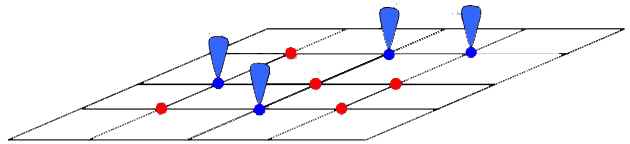
\includegraphics[width=0.45\textwidth]{figures/Langmuir_Adsorption_Model.jpg}
\caption{A simple graphic representation of the Langmuir adsorption model, where the red dots signify the unoccupied area, the blue points the occupied area.}
\end{figure}

Langmuir supposed that the adsorption rate is proportionl to the pressure of gas A and the area on the surface which haven't been occupied, while the desorption rate is proportional to the area occupied, which is shown by
\begin{equation}
k_{ad} p S_0 = k_{de} S_1
\end{equation}
where $k_{ad},k_{de}$ represent the reaction rate constant of the adsorption and the desorption respectively, $S_0,S_1$ the unoccupied and the occupied area, and $p$ the pressure of gas A in bulk phase.

Define the occupied percentage $\theta$
\begin{equation}
\theta = \frac{S_1}{[S]} = \frac{S_1}{S_0+S_1} = \frac{k_{ad}p}{k_{ad}p+k_{de}}
\end{equation}
and the adsorption equilibrium constant $K=\frac{k_{ad}}{k_{de}}$, then
\begin{equation}
\theta = \frac{Kp}{1+Kp}
\end{equation}


\section{BET: multi-molecular equilibrium}
\begin{figure}
\centering
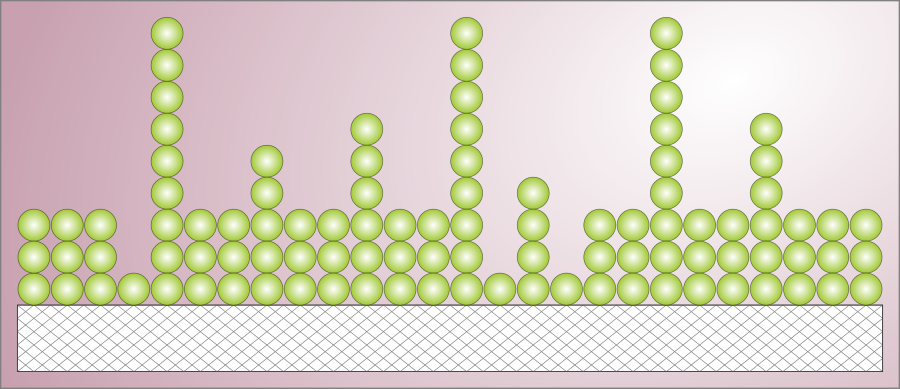
\includegraphics[width=0.45\textwidth]{figures/900px-BET_Multilayer_Adsorption.svg.png}
\caption{Sketch of the multilayered adsorption}
\end{figure}
It is supposed that many layers of adsorbed molecules can be formed on the surface of condensed substance, and $s_i$ is defined as the surface area that covered by $i$ layers of adsorbed molecules. When considering monolayer system, it is derived from the Langmuir's equation that
\begin{equation}
a_1 p s_0 = b_1 s_1 e^{-E_1/RT}
\label{firstlayer}
\end{equation}
where the term $e^{-E_1/RT}$ is separated from $K$ in the Langmuir's equation w.r.t. the Boltzmann distribution achieved between the adsorbed molecules and those in the bulk phase. For another system including only two layers of adsorbed molecules, the equilibrium is given by
\begin{equation}
a_2 p s_1 + b_1 s_1 e^{-E_1/RT} = b_2 s_2 e^{-E_2/RT} + a_1 p s_0
\end{equation}
with each term representing condensation on the first layer, evaporation from the first layer, evaporation from the second layer and condensation on the first layer, with $a_2,\, b_2,\, E_2$ similarly defined to $a_1,\, b_1$ and $E_1$. Considering that (\ref{firstlayer}) still holds in this system for the first layer, it is easily derived that
\begin{equation}
a_2 p s_1 = b_2 s_2 e^{-E_2/RT}
\end{equation}
Similar mechanism can be applied for an arbitrary index $i$, namely
\begin{equation}
a_i p s_{i-1} = b_i s_i e^{-E_i/RT}
\end{equation}
or
\begin{equation}
p s_{i-1} = g_i s_i e^{-E_i/RT}
\end{equation}
The total surface area is given by
\begin{equation}
A=\sum_{i=0}^{\infty} s_i
\end{equation}
and the total volume adsorbed is 
\begin{equation}
v = v_0 \sum_{i=0}^{\infty} i \cdot s_i
\end{equation}
where $v_0$ is the volume of gas adsorbed on unit area of the adsorbent surface when it is covered with a complete unimolecular layer of adsorbed gas. Then
\begin{equation}
\frac{v}{Av_0} = \frac{v}{v_0} = \frac{\sum_{i=0} i\cdot s_i}{\sum s_i}
\end{equation}
It is assumed that $E_i = E_j =E_L, g_i = g_j = g$ for $i,j \geq 2$, in the consideration of the similarity among these layers, and $s_i$ is given by
\begin{equation}
s_0 = c x^i s_0
\end{equation}
where $x = (p/g) e^{E/RT}, c = g g_1 e^{(E_1-E_L)/RT}$. Thus
\begin{equation}
\frac{v}{v_m} = \frac{c \sum_{i=1}^\infty i x^i}{1+ c \sum_{i=1}^\infty x^i}
\end{equation}
Then
\begin{equation}
\frac{v}{v_m} = \frac{cx}{(1-x)(1-x+cx)}
\label{BETmeta}
\end{equation}
w.r.t. the fact that
\begin{equation}
\sum_{i=1}^{\infty} x^i = \frac{x}{1-x} 
\end{equation}
(\ref{BETmeta}) indicates that endless adsorption will occur if $x \rightarrow 1$, which is evidently the result of $p \geqslant p_0$, $p_0$ representing the saturated vapor pressure of the adsorbed substance. Considering that $x \propto p$, it is assumed that
\begin{equation}
x= \frac{p}{p_0}
\end{equation}
Then (\ref{BETmeta}) is reduced to
\begin{equation}
\frac{v}{v_m} = \frac{c p}{(p_0-p)\left[1+(c-1)\frac{p}{p_0}\right]}
\end{equation}
or its linear form
\begin{equation}
\frac{c p}{V(p_0-p)} = \frac{1}{V_m}\left[1+(c-1)\frac{p}{p_0}\right]
\end{equation}

\section{Adsorption in the thermodynaic equilibrium perspective}
BET theory is based on dynamical equilbrium achieved between the adsorption and the desorption of the adsorbed species along with the assumption of indifference among the adduction energy and reaction rate constant $g_i$ between layers, which lacks theoretical evidence. Based on his collaborated work with Kai Gu\cite{shi2018high}, Kaihang Shi along with Shicheng Li established a statistical mechanical model combined with Monte Carlo method to provide computational analysis of the adsorption process\footnotetext{This work is still not published}.

If the adsorption between monolayer and gas phase (bulk phase) reaches an equilibrium, the chemical potentials of two phases must be equal:
\begin{equation}
	\mu_\text{bulk} = \mu_\text{ads}
\end{equation}
and the chemical potential of adsorbed phase is contributed by two parts:
\begin{equation}
	\mu_\text{ads} = \mu_\text{2D} + \mu_\text{w}
\end{equation}
where $\mu_\text{w}$ represents the contribution of chemical potential from the adsorbed wall, and $\mu_\text{2D}$ the chemical potential of the 2D monolayer. Regarding the adsorbed molecules packed hexagonally and interact with each other according to two-dimensional Lennard-Jones equation, the total specific configurational energy is given by
\begin{align}
	U _ { 0 } ^ { * } = &\lim _ { L , M \rightarrow \infty } \frac { 2 } { ( L + 1 ) ( M + 1 ) } \nonumber\\ & \sum _ { i , j} ^ { L , M } \sum _ { l , m} ^ { L , M } \left[ \left( \frac { 1 } { \left\| \mathbf { r } _ { i , j } ^ { * } - \mathbf { r } _ { l , m } ^ { * } \right\| } \right) ^ { 12 }- \left( \frac { 1 } { \left\| \mathbf { r } _ { i , j } ^ { * } - \mathbf { r } _ { l , m } ^ { * } \right\| } \right) ^ { 6 } \right]
\end{align}
where $||*||$ is defined as the norm, and $r_{i,j}^*$ is defined as
\begin{equation}
\mathbf { r } _ { i , j } ^ { * } = r _ { 0 } ^ { * } \left[ \left( i + \frac { 1 } { 2 } j \right) \mathbf { e } _ { x } + \frac { \sqrt { 3 } } { 2 } j \mathbf { e } _ { y } \right]
\end{equation}
which matches the hexagonal alignment of the molecules, with $r_0^* = r_0/\sigma$ to simplify the form. The pressure at is further defined,
\begin{equation}
	P _ { 2 D , T = 0 } ^ { * } = \left( \rho _ { 2 D } ^ { * } \right) ^ { 2 } \left( \frac { \partial U _ { 0 } ^ { * } } { \partial \rho _ { 2 D } ^ { * } } \right)
\end{equation}
where $\rho_{2D}^*$ is the density of the molecules in two dimensional form. With these the chemical potential can be deduced. Using similar method the chemical potential of the wall can be given as a function of $\sigma_\text{ad-solid},\, \varepsilon_\text{ad-solid},\,\lambda\sigma_\text{ad-ad}$ and $T$, representing the colision diameter between the adsorbed molecules and the wall, the adsorbate-surface energy depth, the depth of the monolayer and temperature respectively. Computational analysis reveals that the cross-sectional area of each molecule, as well as the density of the layer, is highly dependent on the interaction between the wall and the adsorbed molecules, which is neglected in the BET theory.


\section{Methodology}
The use of nitrogen adsorption becomes one of the most widely-used method for the characterization of porous materials. The earliest reported studies of the adsorption nitrogen and other gases at liquid air temperature ($\sim$88 K) appear to have been made by Dewar and Ramsay in the course of their investigations of the composition of the atmosphere and the separation of the noble gases.\cite{SING20013}

Gas adsorption manometry is the method generally
used for the determination of adsorption
isotherms of nitrogen at the temperature of liquid
nitrogen ($\sim$77 K). This type of approach was
known as a `volumetric determination' (or alternatively
as the `BET volumetric method') since it
originally involved the measurement of gas volumes,
before and after adsorption. However, it
has been pointed out that it is no longer
appropriate to use the term `volumetric' since the
amount adsorbed is now generally evaluated by
measuring the change of gas pressure, rather than
a change in gas volume.

Two different operational procedures can be
used for the determination of the adsorption
isotherm. The conventional technique makes use
of a discontinuous, point-by-point procedure.
Successive amounts of the adsorptive are introduced
and at each stage the system is allowed
sufficient time to attain equilibrium, which of
course corresponds to a series of single points
on the adsorption isotherm. The continuous approach
is more recent and is dependent on the
principle of `quasi-equilibrium'. In this
case, the introduction of the adsorptive must be
slow enough to provide a continuous `equilibrium'
isotherm (i.e. with an infinite number of
points). If properly used, the continuous manometric
procedure has the great advantage that it
is possible to reveal inconspicuous features (e.g.
sub-steps), which may not be detectable by the
discontinuous method.

The aims of outgassing are two-fold —
(a) to reach a well-defined intermediate state by
the removal of physisorbed molecules; (b) to
avoid any drastic change as a result of ageing
or surface modification. Conventional vacuum
outgassing is the generally preferred technique,
but with fine powders, there is always a risk of
spurting. Spurting can be avoided and changes
in the adsorbent minimised by controlling the
rate of outgassing by the application of a form
of controlled rate thermal analysis, CRTA,
which is also termed `sample controlled thermal
analysis'.

\section{Pore size analysis}
\subsection{The classical approach}
Capillary condensation is generally responsible
for the filling of mesopores and macropores (i.e.
pores of width, $w\geq$2 nm). However, capillary
condensation is a secondary process since it is
always preceded by multilayer adsorption on the
pore walls. Thus, the onset of capillary
condensation is indicated by an upward
deviation from the corresponding multilayer
(Type II) isotherm and the process is complete
if a plateau is attained at higher $p/p_0$. Since
macropore ($w \geq$50 nm) filling occurs only at
very high $p/p_0$, the characteristic Type IV
isotherm shape is generally associated with
mesoporous adsorbents. The mesopore capacity
is the amount adsorbed at the plateau and the
mesopore volume is then obtained by assuming
the condensate density to be that of liquid
nitrogen (i.e. 0.808 $\mathrm{g/cm^{-3}}$).

According to the classical approach, a
corrected form of the Kelvin equation can be
used to evaluate the pore width from the pore
filling pressure:
\begin{equation}
 	\ln{\frac{p}{p_0}} = \frac{2\gamma V_m}{rRT}
 \end{equation}
  where $r$ is the radius of the droplet. 
  It is necessarily assumed that the
pores are rigid and all of the same simple shape
(cylinders or parallel-sided slits) and that the
meniscus curvature is dependent on the
dimensions of the pores. In the computation of
the mesopore size distribution, allowance must
be made for the effect of the multilayer
thickness in reducing the dimensions of the free
pore space available for capillary condensation.

\subsection{Density functional formulation}
Over the past few years density functional theory
(DFT), which in the refined form of nonlocal
density functional theory (NLDFT), has become
an important tool for the characterisation of
porous materials. The approach is based
on the established principles of statistical mechanics
and necessarily assumes a model solid structure
and pore topology. The pores of different size
are assumed to be all of the same regular shape
(e.g. cylinders or slits) and generally each pore is
assumed to behave independently. The adsorbate
is pictured as an inhomogeneous fluid, which is
characterised by its density profile across the pore.
According to the DFT theory, the solid–fluid and
fluid–fluid interactions control the pore filling,
which may take the form of micropore filling or
capillary condensation. If the adsorbent surface is
assumed to be homogeneous, the derived energetic
heterogeneity can be attributed to the pore
size distribution. The interpretation is evidently
more complicated when the energetic heterogeneity
is associated with both the surface chemistry
and the pore structure.

With the availability of commercial software,
DFT has become user friendly. However,
it must be kept in mind that it is of limited value
unless the solid and surface structures are known
and the pores are all of a similar, well-defined,
shape. Much attention has been given so far to
assemblies of slits between graphitic slabs, which
are taken to represent porous carbons.
Another favoured structure is an assemblage of
non-intersecting tubular pores as in MCM-41.



\bibliography{References}

\end{document}
